%%%%%%%%%%%%%%%%%%%%%%%%%%%%%%%%%%%%%%%%%%%%%%%%%%%%%%%%%%%%%%%%%%%%%%%%%%%%%%%%%%%%%%%%%%%%%%%%%%%%

\documentclass{article}

%%%%%%%%%%%%%%%%%%%%%%%%%%%%%%%%%%%%%%%%%%%%%%%%%%%%%%%%%%%%%%%%%%%%%%%%%%%%%%%%%%%%%%%%%%%%%%%%%%%%

\usepackage{tikz}
\usetikzlibrary{calc,positioning,shapes,shadows,arrows,decorations,decorations.pathmorphing,external}
\tikzexternalize % activate! & run "pdflatex -shell-escape test.tex"
\usepackage{pgffor}

%%%%%%%%%%%%%%%%%%%%%%%%%%%%%%%%%%%%%%%%%%%%%%%%%%%%%%%%%%%%%%%%%%%%%%%%%%%%%%%%%%%%%%%%%%%%%%%%%%%%

\begin{document}
%%%%%%%%%%%%%%%%%%%%%%%%%%%%%%%%%%%%%%%%%%%%%%%%%%%%%%%%%%%%%%%%%%%%%%%%%%%%%%%%
\tikzsetnextfilename{figure-hdf5-file-system}
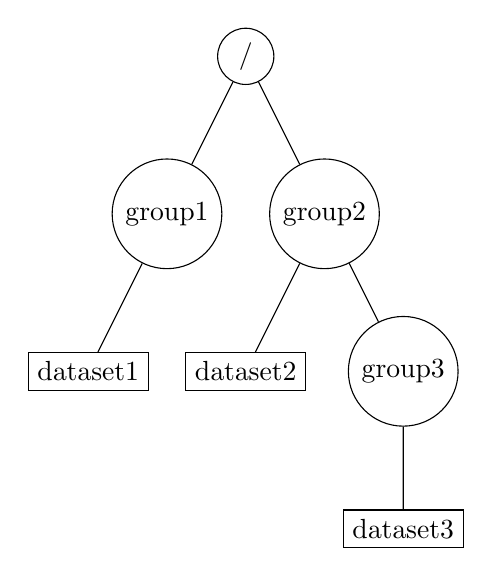
\begin{tikzpicture}
  \node[circle,draw] {/}
    [level distance=20mm, sibling distance=20mm]
    child {node[circle,draw] {group1}
      child {node[rectangle,draw] {dataset1}}
      child[missing]
    }
    child {node[circle,draw] {group2}
      child {node[rectangle,draw] {dataset2}}
      child {node[circle,draw] {group3}
        child {node[rectangle,draw] {dataset3}}
      }
    };
\end{tikzpicture}
%%%%%%%%%%%%%%%%%%%%%%%%%%%%%%%%%%%%%%%%%%%%%%%%%%%%%%%%%%%%%%%%%%%%%%%%%%%%%%%%
\tikzsetnextfilename{figure-hdf5-pipeline}
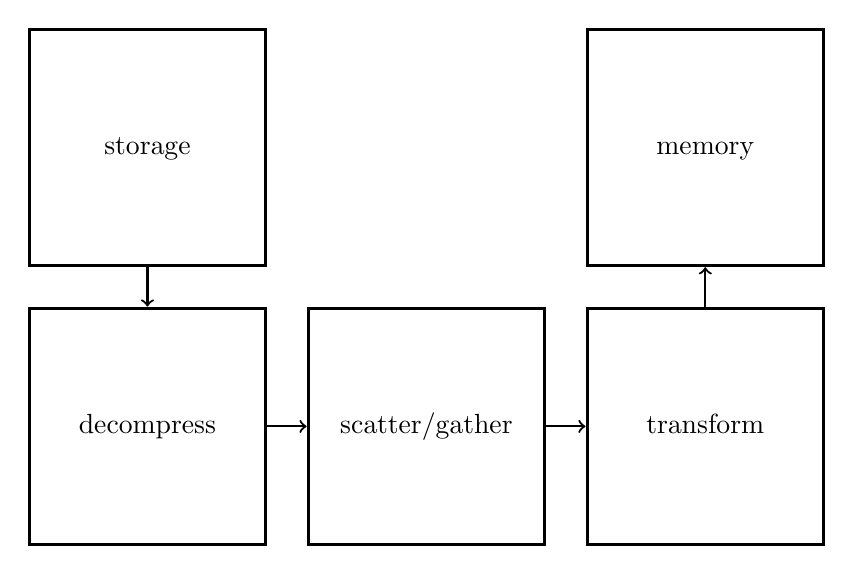
\begin{tikzpicture}[node distance=5mm and 5mm,
  text height=1.5ex,text depth=.25ex,
  thick,
  nodestyle/.style={
    rectangle,
    draw=black,
    minimum size=30mm,
    very thick,
  }]
\node[nodestyle] (storage) {storage};
\node[nodestyle] (decompress) [below=of storage] {decompress};
\node[nodestyle] (scatterGather) [base right=of decompress] {scatter/gather};
\node[nodestyle] (transform) [base right=of scatterGather] {transform};
\node[nodestyle] (memory) [above=of transform] {memory};
\path (storage) edge[->] (decompress)
  (decompress) edge[->] (scatterGather)
  (scatterGather) edge[->] (transform)
  (transform) edge[->] (memory);
\end{tikzpicture}
%%%%%%%%%%%%%%%%%%%%%%%%%%%%%%%%%%%%%%%%%%%%%%%%%%%%%%%%%%%%%%%%%%%%%%%%%%%%%%%%
\tikzsetnextfilename{figure-dataset}
\def\BoxWidth{6}
\def\BoxHeight{.8*\BoxWidth}
\begin{tikzpicture}[yscale=-1]
  \foreach \x in {0,1}
  \foreach \y in {0,1}
  {
    \node (a) at (\x*\BoxWidth,\y*\BoxHeight) {\huge tile (\x,\y)};
    \foreach \i in {-1,1}
    \foreach \j in {-1,1}
    {
      \node (b) at ($(a) - .25*(\i*\BoxWidth,\j*\BoxHeight)$) {}; % {chunk (\x,\y,\i,\j)};
      \draw[dotted] ($(b) - .25*(\BoxWidth,\BoxHeight)$) rectangle ++($.5*(\BoxWidth,\BoxHeight)$);
    }
    \draw[very thick] ($(a) - .5*(\BoxWidth,\BoxHeight)$) rectangle ++(\BoxWidth,\BoxHeight);
  }
\end{tikzpicture}
%%%%%%%%%%%%%%%%%%%%%%%%%%%%%%%%%%%%%%%%%%%%%%%%%%%%%%%%%%%%%%%%%%%%%%%%%%%%%%%%
\tikzsetnextfilename{figure-linear-dataset}
\def\BoxWidth{6}
\def\BoxHeight{.5*\BoxWidth}
\def\Margin{2}
\def\Bottom{3*\BoxHeight}
\def\BottomMargin{\Bottom+\Margin}
\begin{tikzpicture}[yscale=-1]
  % \draw[dashed] (0,0) -- (0,-\Margin);
  % \draw[solid] (0,-\Margin) -- (\BoxWidth,-\Margin);
  % \draw[dashed] (\BoxWidth,-\Margin) -- (\BoxWidth,0);
  % \draw[dashed] (0,\Bottom) -- (0,\BottomMargin);
  % \draw[solid] (0,\BottomMargin) -- (\BoxWidth,\BottomMargin);
  % \draw[dashed] (\BoxWidth,\BottomMargin) -- (\BoxWidth,\Bottom);
  \draw[decorate, decoration={random steps,segment length=3pt,amplitude=1pt}]
  (0,0) -- (0,-\Margin) -- (\BoxWidth,-\Margin) -- (\BoxWidth,0)
  (0,\Bottom) -- (0,\BottomMargin) -- (\BoxWidth,\BottomMargin) -- (\BoxWidth,\Bottom);
  \draw[<->] (0,-.5) -- node[above] {W} ++(\BoxWidth,0);
  \coordinate (p) at (-.5,0);
  \draw[->] (p) -- (0,0);
  \node[anchor=east] at (p) {$p(r,c)=(r\,C+c)(N_w\,H)$};
  \coordinate (pw1) at ($(0,\BoxHeight) + (-.5,0)$);
  \draw[->] (pw1) -- (0,\BoxHeight);
  \node[anchor=east] at (pw1) {$p(r,c,w)=p(r,c)+w\,H$};
  \foreach \w in {0,...,2}
    {
      \coordinate (a) at (0,\w*\BoxHeight);
      \draw (a) rectangle ++(\BoxWidth,\BoxHeight);
      \draw ($(a) + (.5*\BoxWidth,.5*\BoxHeight)$) node {w\w};
      \foreach \i in {-1,1}
      \foreach \j in {-1,1}
      {
        \coordinate (b) at ($(a) + .5*(\BoxWidth,\BoxHeight) - .25*(\i*\BoxWidth,\j*\BoxHeight)$);
        \draw[dotted] ($(b) - .25*(\BoxWidth,\BoxHeight)$) rectangle ++($.5*(\BoxWidth,\BoxHeight)$);
      }
    }
\end{tikzpicture}
\end{document}

%%%%%%%%%%%%%%%%%%%%%%%%%%%%%%%%%%%%%%%%%%%%%%%%%%%%%%%%%%%%%%%%%%%%%%%%%%%%%%%%%%%%%%%%%%%%%%%%%%%%
%%% Local Variables: 
%%% mode: latex
%%% TeX-master: t
%%% End: 
%%%%%%%%%%%%%%%%%%%%%%%%%%%%%%%%%%%%%%%%%%%%%%%%%%%%%%%%%%%%%%%%%%%%%%%%%%%%%%%%%%%%%%%%%%%%%%%%%%%%
